\section{Parameters}

Un parametro, rappresentato dalla classe \verb|Parameter|, rappresenta un valore con determinate caratteristiche che viene utilizzato in svariati contesti all'interno di AULOS.
\begin{lstlisting}[caption={Parameter.cs},style=sharpCode]
public class Parameter
{
    public Parameter();
    public string Code { get; set; }
    public ParameterDescriptor Descriptor { get; set; }
    public string Value { get; set; }
    public List<Parameter> SubParameters { get; set; }
    public string DescriptorCode { get; set; }
    public StandardParameterType Type { get; set; }
    public Parameter GetSubParameter(string code);
}
\end{lstlisting}
\begin{itemize}
\item \verb|Code| è l'identificativo univoco del parametro;
\item \verb|Descriptor| è il descrittore del parametro, utilizzato per creare il parametro lato frontend;
\item \verb|Value| è il valore del parametro;
\item \verb|SubParameters| sono i sottoparametri del parametro (un parametro può rappresentare un'aggregazione di altri parametri);
\item \verb|Type| rappresenta il tipo del valore rappresentato dal parametro.
\end{itemize}
La classe \verb|ParameterDescriptor| è così formata:
\begin{lstlisting}[caption={ParameterDescriptor.cs},style=sharpCode]
public class ParameterDescriptor
{
    public ParameterDescriptor();        
    public string Code { get; set; }
    public string ShortText { get; set; }
    public string LongText { get; set; }
    public StandardParameterType Type { get; set; }
    public string ContentType { get; set; }
    public ParameterEditor Editor { get; set; }
    public string MeasureUnit { get; set; }
    public string DefaultValue { get; set; }
    public string Format { get; set; }
    public ParameterValidator Validator { get; set; }
    public List<ParameterDescriptor> SubParameters { get; set; }
    public ParameterDescriptor ItemDescriptor { get; set; }
    public List<string> ItemDescriptorCodes { get; set; }
    public string WriteEnabledConditionCode { get; set; }
    public string VariantType { get; set; }
}
\end{lstlisting}
L'attributo \verb|Editor|, istanza della classe \verb|ParameterEditor|, descrive l'eventuale \verb|Editor| utilizzato lato frontend per permettere la modifica del parametro da parte dell'utente.

\subsection{Parameter Editor}
La classe \verb|ParameterEditor| è così composta:
\begin{lstlisting}[caption={ParameterEditor.cs},style=sharpCode]
public class ParameterEditor
{
    public ParameterEditor();
    public string Type { get; set; }
    public string Path { get; set; }
    public dynamic Options { get; set; }
}
\end{lstlisting}
\begin{itemize}
\item \verb|Type| è il codice univoco dell'\verb|Editor| memorizzato lato frontend;
\item \verb|Path| è il path dove AULOS dovrà cercare l'\verb|Editor|;
\item \verb|Options| sono le eventuali opzioni che l'\verb|Editor| può avere.
\end{itemize}

\subsubsection{Custom Editors}
AULOS fornisce diversi \verb|Editor| per permettere all'utente di modificare i parametri, ma è possibile crearne di nuovi per casi d'uso più specifici. Un \verb|Editor| è un \verb|Component| Angular che va registrato all'interno dell'\verb|EditorFactory| attraverso il metodo \verb|register| .\\
\begin{lstlisting} [caption={dashboard-parameter-editors.module.ts},style=javascriptCode]
export class DashboardParameterEditorsModule {

    ...

    public static appInitializer(): () => Promise<void> {
        const result = (): Promise<void> => {
            return new Promise((resolve, reject) => {
            
                ...
                
                EditorFactory.register(
                    EDITOR_BASE_PATH,
                    'DropdownEditor',
                    DropdownEditorComponent);
                resolve();
            });
        };
        return result;
    }
}
\end{lstlisting}
Il \verb|template| dell'\verb|Editor Component| contiene tre direttive strutturali (\verb|aulosEditorSmallTemplate|, \verb|aulosEditorCompactTemplate| e \verb|aulosEditorExpandedTemplate|), le quali contengono il codice HTML che deve essere visualizzato a seconda dello spazio in cui è contenuto l'\verb|Editor|.
\begin{lstlisting}[caption={source-editor.component.html},style=html]
<aulos-editor-layout [editorConfiguration]="editorConfiguration">
  <ng-template aulosEditorSmallTemplate>
    <div class="input-group" [class.hidden]="disabled">
      <input type="text" 
        class="form-control form-control-sm is-invalid"
        [placeholder]="mySelection[0] ? 
        mySelection[0] : 
        'Choose data source...'  | aulosTranslate" 
        disabled readonly>
      <button class="btn btn-sm btn-icon" [disabled]="disabled" (click)="showExpandedModal()">
        <i class="fontaulos fontaulos-edit"></i>
      </button>
    </div>
  </ng-template>
  <ng-template aulosEditorCompactTemplate>
    <div class="input-group" [class.hidden]="disabled">
      <input 
      type="text" 
      class="form-control is-invalid" 
      [placeholder]="this.model.value ? 
      this.model.value : 
      'Choose data source...'  | aulosTranslate" 
      disabled
        readonly>
      <button class="btn btn-icon" [disabled]="disabled" (click)="showExpandedModal()">
        <i class="fontaulos fontaulos-edit"></i>
      </button>
    </div>
  </ng-template>
  <ng-template aulosEditorExpandedTemplate>
    <kendo-grid
              [data]="gridData"
              [style.maxlength]="501"
              [filterable]="true"
              [filter]="state.filter"
              [selectable]="selectableSettings"
              [sortable]="true"
              style="padding-top: 2%; padding-bottom: 5%;"
              (dataStateChange)="dataStateChange($event)"
              kendoGridSelectBy="sourceCode"
              [selectedKeys]="tmpSelection"
            >
            <kendo-grid-checkbox-column width="60%"></kendo-grid-checkbox-column>
            <kendo-grid-column field="sourceCode" filter="text"></kendo-grid-column>
            <kendo-grid-column field="shortText" filter="text"></kendo-grid-column>
            <kendo-grid-column field="longText" filter="text"></kendo-grid-column>
            <ng-template kendoGridNoRecordsTemplate>
              No sources available.
           </ng-template>
          </kendo-grid>
  </ng-template>
</aulos-editor-layout>
\end{lstlisting}
È necessario che l'\verb|Editor Component| estenda \verb|BaseEditorComponent|, classe che offre delle funzionalità di interfacciamento con AULOS, e che presenti la logica necessaria alla modifica del parametro a esso associato.

\subsection{Utilizzo dei parametri nell'applicativo}
Nell'applicativo, il parametro svolge una duplice funzione:
\begin{itemize}
\item permette di gestire la configurazione di un widget lato frontend;
\item viene utilizzato per specificare dei filtri da applicare in fase di ottenimento dei dati.
\end{itemize}
La classe Widget e le sue estensioni nell'applicazione frontend hanno la responsabilità di gestire i parametri legati a un widget. Questi parametri possono rappresentare un attributo grafico del widget, un valore della sua configurazione oppure un filtro da applicare ai dati da visualizzare.
\begin{figure}[h!]
\begin{center}
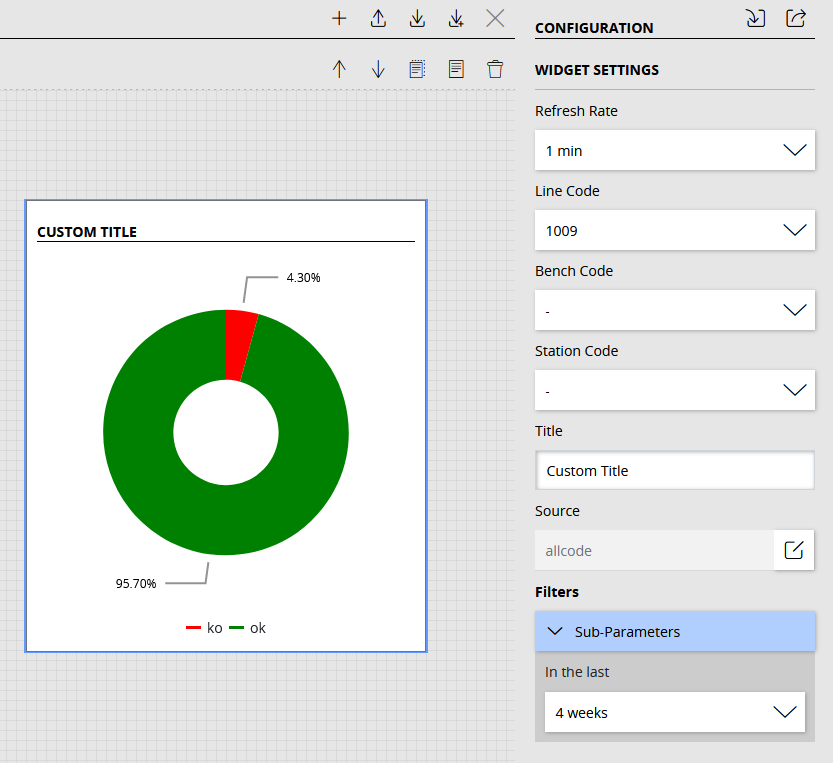
\includegraphics[scale=0.5]{parameters_example}\\
\caption{Possibile configurazione del widget PieChart}
\end{center}
\end{figure}
\subsubsection{Filter Parameters}
Data la capacità dei parametri di poter rappresentare dati eterogenei, sono stati utilizzati per rappresentare i possibili filtri di una \textit{query}.\\
I parametri \verb|filters| vengono generati attraverso dei \verb|ParameterDescriptor|, presi con una chiamata REST [\ref{chap:frontend}] dopo che è stata definita una source.
\begin{lstlisting}[caption={initSourceCalls, base-widget.ts},style=javascriptCode]
private async initSourceCalls() {

	...
	
        await this.sourceParameter.valueChanges.subscribe(sourceCode => {
            this.sourceSet = true;
            this.widgetService.getSourceProperties(sourceCode).subscribe(sourceProperties => {
                this.metadata = sourceProperties.metadata;
                this.setFilters(sourceProperties.filters);
                this.notifyStateChanged();
            });
        });
        this.initSource();
}
\end{lstlisting}